%%%%%%%%%%%%%%%%%%%%%%%%%%%%%%%%%%%%%%%%%%%%%%%%%%%%%%%%%%%%%%%%%%%%%%
%%  Copyright by Wenliang Du.                                       %%
%%  This work is licensed under the Creative Commons                %%
%%  Attribution-NonCommercial-ShareAlike 4.0 International License. %%
%%  To view a copy of this license, visit                           %%
%%  http://creativecommons.org/licenses/by-nc-sa/4.0/.              %%
%%%%%%%%%%%%%%%%%%%%%%%%%%%%%%%%%%%%%%%%%%%%%%%%%%%%%%%%%%%%%%%%%%%%%%

\newcommand{\commonfolder}{../../common-files}

\documentclass[11pt]{article}

\usepackage[most]{tcolorbox}
\usepackage{times}
\usepackage{epsf}
\usepackage{epsfig}
\usepackage{amsmath, alltt, amssymb, xspace}
\usepackage{wrapfig}
\usepackage{fancyhdr}
\usepackage{url}
\usepackage{verbatim}
\usepackage{fancyvrb}
\usepackage{adjustbox}
\usepackage{listings}
\usepackage{color}
\usepackage{subfigure}
\usepackage{cite}
\usepackage{sidecap}
\usepackage{pifont}
\usepackage{mdframed}
\usepackage{textcomp}
\usepackage{enumitem}
\usepackage{hyperref}


% Horizontal alignment
\topmargin      -0.50in  % distance to headers
\oddsidemargin  0.0in
\evensidemargin 0.0in
\textwidth      6.5in
\textheight     8.9in 

\newcommand{\todo}[1]{
\vspace{0.1in}
\fbox{\parbox{6in}{TODO: #1}}
\vspace{0.1in}
}


\newcommand{\unix}{{\tt Unix}\xspace}
\newcommand{\linux}{{\tt Linux}\xspace}
\newcommand{\minix}{{\tt Minix}\xspace}
\newcommand{\ubuntu}{{\tt Ubuntu}\xspace}
\newcommand{\setuid}{{\tt Set-UID}\xspace}
\newcommand{\openssl} {\texttt{openssl}}


\pagestyle{fancy}
\lhead{\bfseries SEED Labs}
\chead{}
\rhead{\small \thepage}
\lfoot{}
\cfoot{}
\rfoot{}


\definecolor{dkgreen}{rgb}{0,0.6,0}
\definecolor{gray}{rgb}{0.5,0.5,0.5}
\definecolor{mauve}{rgb}{0.58,0,0.82}
\definecolor{lightgray}{gray}{0.90}


\lstset{%
  frame=none,
  language=,
  backgroundcolor=\color{lightgray},
  aboveskip=3mm,
  belowskip=3mm,
  showstringspaces=false,
%  columns=flexible,
  basicstyle={\small\ttfamily},
  numbers=none,
  numberstyle=\tiny\color{gray},
  keywordstyle=\color{blue},
  commentstyle=\color{dkgreen},
  stringstyle=\color{mauve},
  breaklines=true,
  breakatwhitespace=true,
  tabsize=3,
  columns=fullflexible,
  keepspaces=true,
  escapeinside={(*@}{@*)}
}

\newcommand{\newnote}[1]{
\vspace{0.1in}
\noindent
\fbox{\parbox{1.0\textwidth}{\textbf{Note:} #1}}
%\vspace{0.1in}
}


%% Submission
\newcommand{\seedsubmission}{
Debe enviar un informe de laboratorio detallado, con capturas de pantalla, para describir lo que ha hecho y lo que ha observado.
También debe proporcionar una explicación a las observaciones que sean interesantes o sorprendentes.
Enumere también los fragmentos de código más importantes seguidos de una explicación. No recibirán créditos aquellos fragmentos de códigos que no sean explicados.}

%% Book
\newcommand{\seedbook}{\textit{Computer \& Internet Security: A Hands-on Approach}, 2nd
Edition, by Wenliang Du. Para más detalles \url{https://www.handsonsecurity.net}.\xspace}

%% Videos
\newcommand{\seedisvideo}{\textit{Internet Security: A Hands-on Approach},
by Wenliang Du. Para más detalles \url{https://www.handsonsecurity.net/video.html}.\xspace}

\newcommand{\seedcsvideo}{\textit{Computer Security: A Hands-on Approach},
by Wenliang Du. Para más detalles \url{https://www.handsonsecurity.net/video.html}.\xspace}

%% Lab Environment
\newcommand{\seedenvironment}{Este laboratorio ha sido testeado en nuestra imagen pre-compilada de una VM con Ubuntu 16.04, que puede ser descargada del sitio oficial de SEED.\xspace}

\newcommand{\seedenvironmentA}{Este laboratorio ha sido testeado en nuestra imagen pre-compilada de una VM con Ubuntu 16.04, que puede ser descargada del sitio oficial de SEED.\xspace}

\newcommand{\seedenvironmentB}{Este laboratorio ha sido testeado en nuestra imagen pre-compilada de una VM con Ubuntu 20.04, que puede ser descargada del sitio oficial de SEED .\xspace}

\newcommand{\seedenvironmentC}{Este laboratorio ha sido testeado en nuestra imagen pre-compilada de una VM con Ubuntu 20.04, que puede ser descargada del sitio oficial de SEED. Sin embargo, la mayoría de nuestros laboratorios pueden ser realizados en la nube para esto Ud. puede leer nuestra guía que explica como crear una VM de SEED en la nube.\xspace}

\newcommand{\seedenvironmentAB}{
Este laboratorio ha sido testeado en nuestras imagenes pre-compiladas de una VM con Ubuntu 16.04 y otra con Ubuntu 20.04, que pueden ser descargadas del sitio oficial de SEED.\xspace}

\newcommand{\nodependency}{Dado que utilizamos contenedores para configurar el entorno de laboratorio, este laboratorio no depende estrictamente de la VM de SEED. Puede hacer este laboratorio utilizando otras máquinas virtuales, máquinas físicas o máquinas virtuales en la nube.\xspace}

\newcommand{\adddns}{You do need to add the required IP address mapping to
the \texttt{/etc/hosts} file.\xspace}






\newcommand{\seedlabcopyright}[1]{
\vspace{0.1in}
\fbox{\parbox{6in}{\small Copyright \copyright\ {#1}\ \ by Wenliang Du.\\
      Este trabajo se encuentra bajo licencia Creative Commons.
       Attribution-NonCommercial-ShareAlike 4.0 International License.
       Si ud. remezcla, transforma y construye a partir de este material,
       Este aviso de derechos de autor debe dejarse intacto o reproducirse de una manera que sea razonable para el medio en el que se vuelve a publicar el trabajo.
       }}
\vspace{0.1in}
}






\lhead{\bfseries SEED Labs -- Laboratorio del Ataque Return-to-libc}

\newcommand{\retFigs}{./Figs}

\def \code#1 {\fbox{\scriptsize{\texttt{#1}}}}

\begin{document}

\begin{center}
{\LARGE Laboratorio del Ataque Return-to-libc }
\end{center}

\seedlabcopyright{2006 - 2020}


% *******************************************
% SECTION
% ******************************************* 
\section{Descripción General}

El objetivo de este laboratorio es que los estudiantes aprendan y ganen experiencia en un tipo de variante de ataque a los buffer overflow; este ataque puede evadir un mecanismo de protección existente que es implementando en la mayoría de los sistemas operativos Linux. La forma tradicional de explotar una vulnerabilidad de buffer overflow es desbordar el buffer con un shellcode malicioso y hacer que el programa explotado haga un salto (jump) al shellcode dentro del stack. Para prevenir este tipo de ataques, algunos sistemas operativos hacen que su stack no sea ejecutable; lo que hará que falle la ejecución del shellcode dentro del mismo.

Desafortunadamente, esta protección no es infalible. Existe una variante para atacar esta vulnerabilidad dadas en los buffer overflows llamada  \textit{Return-to-libc}, que no necesita que el stack sea ejecutable; es más, no usa un shellcode. En su lugar hace que el programa salte (jump) a algún código que ya existe como puede ser la función \texttt{system()} de la librería \texttt{libc}, la cual es cargada en el espacio de memoria del proceso.

En este laboratorio, los estudiantes contarán con un programa con una vulnerabilidad de buffer overflow; su tarea será usar el ataque Return-to-libc para explotar la vulnerabilidad de este programa y finalmente obtener privilegios de root.
Además de esto, los estudiantes serán instruidos en otros tipos de mecanismos de protección implementados en Ubuntu para prevenir ataques de buffer overflow.
Este laboratorio cubre los siguientes tópicos:

\begin{itemize}[noitemsep]
\item Vulnerabilidad de Buffer overflow
\item El Stack Layout en la invocación a una función y el Non-executable stack 
\item Ataque de Return-to-libc y Return-Oriented Programming (ROP)
\end{itemize}


\paragraph{Lecturas y Videos.}
Para una cobertura más detallada en el ataque de return-to-libc puede consultar

\begin{itemize}
\item Capítulos 5 del libro de SEED, \seedbook
\item Sección 5 del curso de SEED en Udemy, \seedcsvideo
\end{itemize}


\paragraph{Entorno de Laboratorio.} \seedenvironmentC


\paragraph{Nota para instructores.}
Los instructores pueden personalizar este laboratorio eligiendo determinados valores para el tamaño del buffer que es usado en el programa vulnerable.
Para más detalles vea la Sección \ref{sec:vulnerable_program}.


% *******************************************
% SECTION
% ******************************************* 
\section{Configuración del Entorno de Laboratorio}


% -------------------------------------------
% SUBSECTION
% ------------------------------------------- 
\subsection{Nota sobre las arquitecturas x86 y x64}

El ataque de return-to-libc es mucho más difícil de realizar usando la arquitectura x64 (64-bits) que usando la arquitectura x86 (32-bits).
Aunque la Máquina Virtual Ubuntu 20.04 de SEED es de 64-bits, se decidió usar programas de 32-bits (la arquitectura x64 es compatible con x86, por lo que programas de 32-bits pueden correr sin problemas en máquinas de 64-bits). En un futuro haremos una versión para 64-bits de este laboratorio.
Para asegurarnos de estar trabajando con un programa de 32-bits, al momento de compilar nuestro programa con \texttt{gcc} usaremos el parámetro \texttt{-m32} que generará un archivo binario de 32-bits.



% -------------------------------------------
% SUBSECTION
% ------------------------------------------- 
\subsection{Desactivando las Contramedidas}

Antes de ejecutar las tareas de los laboratorios en la Máquina Virtual de Ubuntu, hay que tener en cuenta que las distribuciones de Linux implementan diferentes contramedidas para prevenir ataques de buffer overflow, en consecuencia esto dificulta el proceso de explotación de los mismos.
Para simplificar nuestros ataques, procederemos a desactivarlas.


\paragraph{Address Space Randomization.}
Tanto Ubuntu como otros sistemas basados en Linux, usan la randomización de los espacios de memoria (address space randomization), esto hace que las direcciones de memoria tanto en el heap como en el stack sean aleatorias, lo que ocasiona un problema a la hora de calcular las direcciónes de memoria para nuestro ataque ya que contar con estas de antemano es fundamental para que el ataque sea exitoso. 
A continuación se muestra el comando para desactivar esta contramedida:

\begin{lstlisting}
$ sudo sysctl -w kernel.randomize_va_space=0
\end{lstlisting}


\paragraph{El Mecanismo de Protección StackGuard.}
Con el objetivo de prevenir buffer overflows, el compilador \texttt{gcc} implementa un mecanismo de seguridad llamado \textit{StackGuard}. Cuando el StackGuard está activado los ataques de buffer overflow no funcionarán. Podemos desactivar esta protección durante el proceso de compilación de nuestro programa usando el parámetro \emph{-fno-stack-protector}.
A continuación se muestra el comando para desactivar esta protección para el archivo \texttt{example.c}:

\begin{lstlisting}
$ gcc -m32 -fno-stack-protector example.c
\end{lstlisting}


\paragraph{Non-Executable Stack.} Ubuntu solía permitir stacks ejecutables pero esto ha cambiado. La imagen de los programas binarios (y sus librerías compartidas) deben de indicar cuando requieren que el stack sea ejecutable o no, es decir, dentro del encabezado del programa se debe marcar un campo que indica si el stack será o no ejecutable. Este proceso es hecho de forma automática por {\tt gcc} (en sus versiones más recientes), por defecto los stacks son marcados como no ejecutables.
Para poder modificar esto, al momento de compilar un programa se debe hacer de la siguiente forma:

\begin{lstlisting}
For executable stack:
$ gcc -m32 -z execstack  -o test test.c

For non-executable stack:
$ gcc -m32 -z noexecstack  -o test test.c
\end{lstlisting}


Dado que el objetivo de este laboratorio es mostrar que la protección de non-executable stack no es infalible, debería de compilar su programa usando el parámetro {\tt "-z noexecstack"}.


\paragraph{Configurando \texttt{/bin/sh}.} En Ubuntu 20.04, la shell \texttt{/bin/sh} tiene un link simbólico que apunta a la shell \texttt{/bin/dash}.
La shell \texttt{dash} tiene una protección que evita ser ejecutada en un proceso 
\setuid. Si \texttt{dash} es ejecutada en un proceso \setuid, esta hace el cambio del effective user ID al real user ID del proceso que la está ejecutando, eliminando privilegios innecesarios.
Dado que nuestro programa vulnerable es un programa \setuid y nuestro ataque se vale de la función \texttt{system()} para correr el comando de nuestra elección. Esta función no correrá directamente nuestro comando sino que invocará a \texttt{/bin/sh} para realizar esta tarea, por ende será \texttt{/bin/dash} quién eliminirá los privilegios antes de la ejecución del comando a través de la protección built-in anteriormente mencionada, esto hará que nuestro ataque sea más difícil de lograr. Para desactivar esta protección, se debe de crear un link simbólico en la shell \texttt{/bin/sh} hacia otra shell que no tenga esta contramedida.
En nuestra Máquina Virtual Ubuntu 16.04, hemos instalado otra shell llamada \texttt{zsh} que se usará de reemplazo en lugar de \texttt{dash}:

\begin{lstlisting}
$ sudo ln -sf /bin/zsh /bin/sh
\end{lstlisting}

La protección implementada por \texttt{dash} puede ser evadida. Lo haremos en una tarea posterior.



% -------------------------------------------
% SUBSECTION
% -------------------------------------------
\subsection{El Programa Vulnerable}
\label{sec:vulnerable_program}

\begin{lstlisting}[caption={The vulnerable program (\texttt{retlib.c})}]
#include <stdlib.h>
#include <stdio.h>
#include <string.h>

#ifndef BUF_SIZE
#define BUF_SIZE 12
#endif

int bof(char *str)
{
    char buffer[BUF_SIZE];
    unsigned int *framep;

    // Copy ebp into framep
    asm("movl %%ebp, %0" : "=r" (framep));      

    /* print out information for experiment purpose */
    printf("Address of buffer[] inside bof():  0x%.8x\n", (unsigned)buffer);
    printf("Frame Pointer value inside bof():  0x%.8x\n", (unsigned)framep);

    strcpy(buffer, str);   (*@\reflectbox{\ding{222}} \textbf{buffer overflow!} @*)

    return 1;
}

int main(int argc, char **argv)
{
   char input[1000];
   FILE *badfile;

   badfile = fopen("badfile", "r");
   int length = fread(input, sizeof(char), 1000, badfile);
   printf("Address of input[] inside main():  0x%x\n", (unsigned int) input);
   printf("Input size: %d\n", length);

   bof(input);

   printf("(^_^)(^_^) Returned Properly (^_^)(^_^)\n");
   return 1;
}

// This function will be used in the optional task
void foo(){
    static int i = 1;
    printf("Function foo() is invoked %d times\n", i++);
    return;
}
\end{lstlisting}

El programa anterior tiene una vulnerabilidad de buffer overflow. Este programa empieza leyendo un input de más de \texttt{1000} bytes de un archivo llamado \texttt{badfile}, este pasa los datos a la función \texttt{bof()} que los copia en su buffer interno a través de la función \texttt{strcpy()}.
Debido a que el buffer interno de la función \texttt{bof()} tiene un tamaño mucho más chico que \texttt{1000}, existe una potencial vulnerabilidad de buffer overflow.

Nuestro código será un programa \setuid cuyo dueño es el usuario root, de esta forma si un usuario normal quiere explotar esta vulnerabilidad de buffer overflow, podría obtener una shell con privilegios de root. 
Cabe notar que el programa obtiene los datos de entrada de un archivo llamado \texttt{badfile} el cual es provisto por los usuarios, de esta forma podemos construir un archivo de tal forma que cuando el programa vulnerable copie su contenido al buffer, se ejecute una root shell.


\vspace{0.1in}
\paragraph{Compilación.} 
Lo primero que haremos será compilar el programa, setearlo con el bit de \setuid y hacer al usuario root dueño del mismo.
No olvide incluir los parámetros \texttt{-fno-stack-protector} (para desactivar la protección de Stackguard) y  \texttt{"-z noexecstack"} (para activar la protección non-executable stack).
Hay que aclarar que el cambio de dueño del archivo debe de hacerse antes de activar el bit de \setuid, de otra forma se desactivará este bit.
Todos estos comandos son provistos en el archivo \texttt{Makefile}. 


\begin{lstlisting}
// Note: N should be replaced by the value set by the instructor
$ gcc -m32 -DBUF_SIZE=N -fno-stack-protector -z noexecstack -o retlib retlib.c
$ sudo chown root retlib           
$ sudo chmod 4755 retlib           
\end{lstlisting}


\paragraph{Para Instructores.}
Para evitar que los estudiantes utilicen las soluciones del pasado (o de aquellas
publicado en Internet), los instructores pueden cambiar el
valor para \texttt{BUF\_SIZE} haciendo que los estudiantes compilen el código usando un valor \texttt{BUF\_SIZE} diferente.
Si no se usa un valor determinado para \texttt{-DBUF\_SIZE} en la compilacióon 
su valor por defecto será \texttt{12} (definido en el programa).
Cuando este valor se modifica, el layout del stack  cambiará y la solución será diferente.
Los estudiantes deben de pedir a sus instructores
el valor de \texttt{N}. Se puede establecer el valor de \texttt{N}
en el archivo \texttt{Makefile} y se puede usar un valor para \texttt{N} entre 10 y 800.



% *******************************************
% SECTION
% ******************************************* 
\section{Tareas de Laboratorio}



% -------------------------------------------
% SUBSECTION
% -------------------------------------------
\subsection{Tarea 1: Encontrar la Direcciónes de las Funciones de \texttt{libc} } 

Cuando se ejecuta un programa en \linux, la librería \texttt{libc} es cargada en memoria. Cuando el address randomization está desactivado, para el programa en cuestión el espacio de direcciones en donde se carga la librería es siempre el mismo (para diferentes programas, el espacio de direcciones donde se carga \texttt{libc} puede variar).
Por lo tanto, podemos encontrar fácilmente la dirección de \texttt{system()} usando una herramienta de debugging como \texttt{gdb}. Es decir, podemos debuguear
el programa \texttt{retlib}. Aunque el programa sea \setuid y su dueño sea el usuario root, con la única exepción que los privilegio se eliminarán (es decir, el effective user ID será el mismo que el real user ID).
Dentro de \texttt{gdb}, necesitamos correr el programa una sóla vez de otra forma el código de la librería no será cargado, esto lo haremos usando el comando \texttt{run}.
Como se ve a continuación se uso el comando \texttt{p} (o \texttt{print}) para mostrar en pantalla la dirección en memoria de las funciones \texttt{system()} y de \texttt{exit()} (la cual la necesitaremos más adelante).


\begin{lstlisting}
$ touch badfile
$ gdb -q retlib     (*@\reflectbox{\ding{217}} Use "Quiet" mode@*)
Reading symbols from ./retlib...
(No debugging symbols found in ./retlib)
gdb-peda$ break main
Breakpoint 1 at 0x1327
gdb-peda$ run
......
Breakpoint 1, 0x56556327 in main ()
gdb-peda$ p system
$1 = {<text variable, no debug info>} (*@\textbf{0xf7e12420}@*) <system>
gdb-peda$ p exit
$2 = {<text variable, no debug info>} (*@\textbf{0xf7e04f80}@*) <exit>
gdb-peda$ quit
\end{lstlisting}

Debe de notar que aunque se trate del mismo programa, si decidimos desactivar el bit \setuid, puede ocurrir que la librería \texttt{libc} no sea cargada en el mismo espacio de direcciones.


\paragraph{Corriendo \texttt{gdb} en modo batch.} Si prefiere correr \texttt{gdb} en modo batch, puede poner los siguientes comandos \texttt{gdb} dentro de un archivo y ejecutar \texttt{gdb} en conjunción con estos comandos:


\begin{lstlisting}
$ cat gdb_command.txt
break main
run
p system
p exit
quit
$ gdb -q -batch -x gdb_command.txt ./retlib
...
Breakpoint 1, 0x56556327 in main ()
$1 = {<text variable, no debug info>} 0xf7e12420 <system>
$2 = {<text variable, no debug info>} 0xf7e04f80 <exit>
\end{lstlisting}
 



% -------------------------------------------
% SUBSECTION
% ------------------------------------------- 
\subsection{Tarea 2: Insertando la cadena de la shell en la memoria}

Nuestra estrategia de ataque es hacer un salto (jump) a la función \texttt{system()} y ejecutar un comando arbitrario. Dado que queremos obtener una shell, nuestro objetivo es que la función \texttt{system()} ejecute el programa \texttt{"/bin/sh"}. Además se debe poner en memoria la cadena que representa el comando \texttt{"/bin/sh"} por lo que tendremos que conocer su dirección (esta dirección debe de ser pasado a la función \texttt{system()}). Existen varias formas de lograr esto, para esta tarea hemos elegido un método que usa variables de entorno.
Los estudiantes pueden probar con otros métodos si lo desean.  

Cuando ejecutamos un programa desde una shell, la shell crea un proceso hijo para ejecutar ese programa y todas las variables que son exportadas en la shell, son heredadas por ese proceso hijo que crea al ejecutar ese nuevo programa, es decir el proceso hijo hereda las variables de entornos exportadas por la shell padre.
Esto nos permite insertar cadenas en el espacio de direcciones del proceso hijo de manera sencilla.
Procederemos a definir una nueva variable shell llamada \texttt{MYSHELL}, dentro de ella pondremos la cadena \texttt{"/bin/sh"}. 
A continuación usando los siguientes comandos podremos verificar que la cadena esta presente en el proceso hijo y es mostrada en pantalla por el comando \texttt{env} que corre dentro del contexto del mismo.

\begin{lstlisting}
$ export MYSHELL=/bin/sh
$ env | grep MYSHELL
MYSHELL=/bin/sh
\end{lstlisting}

Usaremos la dirección de memoria de esta variable como argumento para la llamada a {\tt system()}. La dirección de esta variable puede ser encontrada usando el siguiente programa: 

\begin{lstlisting}
void main(){
   char* shell =  getenv("MYSHELL");
   if (shell) 
      printf("%x\n", (unsigned int)shell);
}
\end{lstlisting}

Compile el código anterior dentro de un binario llamado \texttt{prtenv}. 
Si el address randomization está desactivado, la dirección de memoria de la variable mostrada por \texttt{prtenv} deberá de coincidir por la que se muestra en el programa vulnerable \texttt{retlib}. Puede verificar ubicando el código mostrado anteriormente dentro de \texttt{retlib.c}. 
Sin embargo tenga en cuenta que la longitud del nombre de programa hace la diferencia, es por eso que elejimos 6 caracteres para \texttt{prtenv} como para 
\texttt{retlib}, ambos nombres deben de tener la misma longitud.



% -------------------------------------------
% SUBSECTION
% -------------------------------------------
\subsection{Tarea 3: Lanzando el Ataque}

Ya estamos listos para generar el contenido de nuestro archivo \texttt{badfile}.
Dado que nuestro contenido incluye datos en binario (por ejemplo: las direcciones de las funciones de \texttt{libc}), podemos usar Python para construir el contenido.
A continuación hemos provisto un código genérico con las partes esenciales que deben de ser completadas por ud.


\begin{lstlisting}
#!/usr/bin/env python3
import sys

# Fill content with non-zero values
content = bytearray(0xaa for i in range(300))

X = 0
sh_addr = 0x00000000       # The address of "/bin/sh"
content[X:X+4] = (sh_addr).to_bytes(4,byteorder='little')

Y = 0
system_addr = 0x00000000   # The address of system()
content[Y:Y+4] = (system_addr).to_bytes(4,byteorder='little')

Z = 0
exit_addr = 0x00000000     # The address of exit()
content[Z:Z+4] = (exit_addr).to_bytes(4,byteorder='little')

# Save content to a file
with open("badfile", "wb") as f:
  f.write(content)
\end{lstlisting}
 
Su objetivo es encontrar las tres direcciones de memoria para los valores de \texttt{X}, \texttt{Y}, y \texttt{Z}. 
Si los valores no son los correctos, el ataque fallará. En el informe de laboratorio deberá de explicar como es que obtuvo los valores para {\tt X}, {\tt Y} y {\tt Z}. Explique su razonamiento o si decide utilizar un enfoque de prueba y error, muestre sus pruebas.


\paragraph{Nota sobre \texttt{gdb}.} Si usa \texttt{gdb} para encontrar los valores para \texttt{X}, \texttt{Y}, y \texttt{Z}. Debe saber que el comportamiento de \texttt{gdb} en Ubuntu 20.04 es un tanto diferente al comportamiento que tiene en Ubuntu 16.04. Para ser más preciso, después de establecer el break point en la función \texttt{bof}, en el momento en que \texttt{gdb} se detiene dentro de \texttt{bof()}, este lo hace antes que el registro \texttt{ebp} apunte al stack frame actual, por lo que si se muestra el valor de \texttt{ebp} en este punto, obtendremos el valor \texttt{ebp} del caller y no el valor de \texttt{ebp} de \texttt{bof}. Para solucionar esto debemos de tipear \texttt{next} para que se ejecuten unas cuantas instrucciones más y se detenga una vez que el registro \texttt{ebp} apunte al stack frame de la función \texttt{bof()}.
La segunda edición del libro de SEED está basada en Ubuntu 16.04, por lo que no tiene este último paso de \texttt{next}.


\paragraph{Primera Variación del Ataque:}
Es necesaria la función \texttt{exit()}? Por favor repita el ataque sin incluir la dirección de esta función dentro del archivo \texttt{badfile}. Escriba las observaciones en el informe de laboratorio.


\paragraph{Segunda Variación del Ataque:} 
Después de que su ataque sea exitoso, cambie el nombre el archivo \texttt{retlib} y asegúrese que la longitud del nombre sea diferente a la actual. Por ejemplo puede cambiarlo a \texttt{newretlib}. Repita el ataque (sin cambiar el contenido del archivo {\tt badfile}). 
Tuvo un ataque exitoso o falló? Si falló explique el porque.

% -------------------------------------------
% SUBSECTION
% ------------------------------------------- 
\subsection{Tarea 4: Evadir la Contramedida de la Shell}

El propósito de esta tarea es hacer el ataque de return-to-libc después de activar la contramedida de la shell.
Antes de hacer las tareas 1,2 y 3, hemos cambiado el link simbólico de \texttt{/bin/sh} hacia \texttt{/bin/zsh}, de esta forma hemos pisado el link original que apuntaba a \texttt{/bin/dash}. Esto es porque algunas shells como texttt{dash} y \texttt{bash} poseen una contramedida que elimina los privilegios cuando un procesos \setuid es ejecutado. En esta tarea, vamos a evadir esta contramedida es decir trataremos de obtener una shell con privilegios de root aún cuando \texttt{/bin/sh} apunte a \texttt{/bin/dash}.  
Para cambiar el link simbólico debemos ejecutar:

\begin{lstlisting}
$ sudo ln -sf /bin/dash /bin/sh
\end{lstlisting}

Aunque \texttt{dash} y \texttt{bash} eliminen los privilegios \setuid, no lo harán si son invocadas con parámetro \texttt{-p}. Cuando retornamos de la función \texttt{system}, esta función invoca \texttt{/bin/sh}, pero no usa el parámetro \texttt{-p} por lo que el privilegio \setuid del programa objetivo será eliminado. Existe una funcion que nos permite ejecutar \texttt{"/bin/bash -p"} sin hacerlo a través de la función \texttt{system}, de esta forma podríamos obtener privilegios de root.

Aunque hay varias funciones en la librería libc que nos permiten hacer esto, dentro de la familia de funciones de \texttt{exec()} , incluyendo \texttt{execl()}, \texttt{execle()}, \texttt{execv()}, etc. Usaremos \texttt{execv()}.


\begin{lstlisting}
int execv(const char *pathname, char *const argv[]);
\end{lstlisting}
 
 
Esta función recibe doss argumentos, el primero es la dirección del comando y el segundo es la dirección al arreglo que representa los argumentos de ese comando. Por ejemplo, si queremoos invocar \texttt{"/bin/bash -p"} usando  \texttt{execv}, necesitamos el siguiente esquema:

\begin{lstlisting}
pathname = address of "/bin/bash" 
argv[0]  = address of "/bin/bash"
argv[1]  = address of "-p"
argv[2]  = NULL (i.e., 4 bytes of zero).
\end{lstlisting}
 
Basándonos en las tareas anteriores podemos obtener las direcciones de memorias de las cadenas involucradas para este comando y así poder construir el arreglo \texttt{argv[]} en el stack, obtener su dirección de memoria y estaremos listos para realizar el ataque de return-to-libc. Esta vez retornaremos a la función  \texttt{execv()}.

Hay una trampa en esto. El valor de \texttt{argv[2]} debe de ser cero (un cero que sea un entero de cuatro bytes). Si ponemos cuatros ceros en nuestro input, la función \texttt{strcpy()} detendrá la copia al encontrar el primero cero; haciendo que lo que se copie en el buffer de la función \texttt{bof()} quede incompleto. Esto parece ser un problema, pero recuerde que todo lo que se encuentra en su input está dentro del stack; dentro del buffer de la función \texttt{main()}. Para simplificar esta tarea, hemos configurado el programa vulnerable para que muestre la dirección de memoria de este buffer.
 
De igual forma como se hizo en la tarea 3, necesita construir su input, de esta forma al retornar de la función \texttt{bof()}, esta retornará a \texttt{execv()}, que obtendrá del stack la dirección de la cadena \texttt{"/bin/bash"} y la del arreglo \texttt{argv[]}. Necesita preparar todo en el stack de tal forma que cuando \texttt{execv()} se invoque, pueda ejecutar \texttt{"/bin/bash -p"} y le otorgue una shell con privilegios de root.
Por favor incluya en su informe de laboratorio como se construye este input.



% -------------------------------------------
% SUBSECTION
% -------------------------------------------
\subsection{Tarea 5 (Opcional): Programación Orientada al retorno (Return-Oriented Programming)}

Existen varias formas de resolver el problema de la tarea 4. Otra de las formas que existen es invocar la función \texttt{setuid(0)} antes de que la función \texttt{system()} sea llamada. La función \texttt{setuid(0)} se encarga de establecer el effective user ID y el real user ID a 0, convirtiendo al proceso en un proceso no-\setuid (pero con privilegios de root). Este enfoque nos obliga a encadenar dos funciones. Este enfoque de encadenar multiples funciones al mismo tiempo, se generalizó para poder encadenar multiples piezas de código juntas y es conocido como la Programación Orientada al Retorno o Return-Oriented Programming (ROP).

Usando ROP para resolver la tarea 4 es algo sofisticado y está mas allá de los límites de este laboratorio. Sin embargo, queremos que los estudiantes tengan una idea general sobre ROP, preguntándoles sobre un caso especial de ROP.
En el programa \texttt{retlib.c}, existe una función llamada \texttt{foo()}, la cual nunca es ejecutada en el programa. Esa función es el objetivo de esta tarea. Su trabajo será explotar el buffer overflow de este programa de tal forma que cuando retorne de la función \texttt{bof()} este invoque \texttt{foo()} 10 veces antes de darle una shell con privilegios de root.
En su informe de laboratorio necesitará describir como construyó su input. A continuación se muestra como debería de lucir el output resultante:

\begin{lstlisting}
$ ./retlib
...
Function foo() is invoked 1 times
Function foo() is invoked 2 times
Function foo() is invoked 3 times
Function foo() is invoked 4 times
Function foo() is invoked 5 times
Function foo() is invoked 6 times
Function foo() is invoked 7 times
Function foo() is invoked 8 times
Function foo() is invoked 9 times
Function foo() is invoked 10 times
bash-5.0#   (*@\reflectbox{\ding{222}} Got root shell! @*)
\end{lstlisting}
 
\paragraph{Guías.} Vamos a revisar que hemos hecho en la Tarea 3. Como primera medida hemos ubicado los datos en el stack, de tal manera que cuando el programa retorna de \texttt{bof()}, este hace un salto a la función \texttt{system()} y cuando esta función retorna, el programa salta a la función \texttt{exit()}.
En esta Tarea usaremos una estrategia similar, pero en lugar de hacer el salto a \texttt{system()} y \texttt{exit()}, construiremos los datos en el stack de manera tal que cuando el programa retorne de \texttt{bof}, retornará a  \texttt{foo}; y cuando retorne de \texttt{foo} este retornará nuevamente a \texttt{foo}.
Esto será repetido 10 veces, cuando se retorne por décima vez, esta retornará a la función \texttt{execv()} y nos dará una shell de root.



\paragraph{Lecturas adicionales.} Lo que hemos hecho en esta tarea es un caso especial de ROP. Ud. puede notar que la función \texttt{foo()} no contiene ningún parámetro. Si tuviera parámetros, invocarla 10 veces sería significativamente más complejo. La técnica más genérica de ROP nos permite invocar un número arbitrario de funciones de forma secuencial, permitiendo que cada función tenga múltiples argumentos.
En la segunda edición del libro de SEED se proveen instrucciones detalladas de como usar la técnica genérica de ROP para resolver el problema en la Tarea 4. Esta explicación contiene el llamada a la función \texttt{sprintf()} cuatro veces antes de invocar \texttt{system("/bin/sh")} para obtener una shell de root. Este método es algo complicado y abarca 15 páginas de explicaciones en el libro.



% *******************************************
% SECTION
% ******************************************* 
\section{Guiás: Entiendo el mecanismo de la llamada a una función}


% -------------------------------------------
% SUBSECTION
% ------------------------------------------- 
\subsection{Entendiendo el Stack Layout}


Para enteder como llevar a cabo los ataques de Return-to-libc, necesitamos entender como funciona el stack. Para comprender esto usaremos un pequeño programa en C. Para más información puede consultar el libro de SEED y las lecturas de SEED.


\begin{lstlisting}
/* foobar.c */
#include<stdio.h>
void foo(int x)
{
  printf("Hello world: %d\n", x);
}

int main()
{
  foo(1);
  return 0;
}
\end{lstlisting}

Usaremos {\tt "gcc -m32 -S foobar.c"}  para generar el código ensamblador del programa.
El archivo resultante será {\tt foobar.s} y su contenido será algo así:


\begin{lstlisting}
    ......
  8 foo:
  9         pushl   %ebp
 10         movl    %esp, %ebp
 11         subl    $8, %esp
 12         movl    8(%ebp), %eax   
 13         movl    %eax, 4(%esp)
 14         movl    $.LC0, (%esp)  : string "Hello world: %d\n"
 15         call    printf
 16         leave
 17         ret
    ......
 21 main:
 22         leal    4(%esp), %ecx
 23         andl    $-16, %esp
 24         pushl   -4(%ecx)
 25         pushl   %ebp
 26         movl    %esp, %ebp
 27         pushl   %ecx
 28         subl    $4, %esp
 29         movl    $1, (%esp)
 30         call    foo
 31         movl    $0, %eax
 32         addl    $4, %esp
 33         popl    %ecx
 34         popl    %ebp
 35         leal    -4(%ecx), %esp
 36         ret
\end{lstlisting}
 


% -------------------------------------------
% SUBSECTION
% ------------------------------------------- 
\subsection{Llamando y entrando a {\tt foo()}}

Vamos a concentrarnos en el stack mientras se llama a la función {\tt foo()}. Podemos ignorar lo que hay en el stack antes de esta llamada. Note que en esta explcación se usa el número de lineas y no la dirección de las instrucciones.



\begin{figure}[htb]
	\centering
	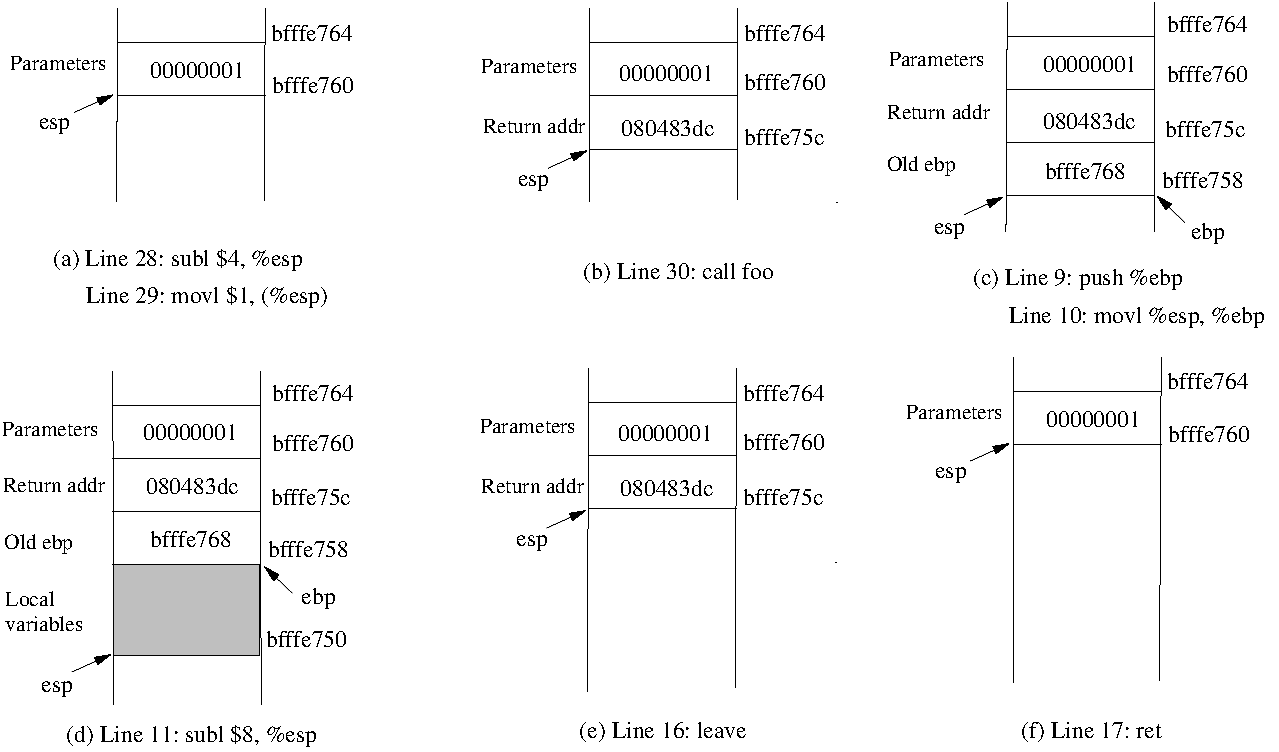
\includegraphics[width=0.95\textwidth]{\retFigs/enter_leave_foo.pdf}
	\caption{Entrando y Saliendo {\tt foo()}}
	\label{fig:enter_leave_foo}
\end{figure}


\begin{itemize}
\item \textbf{Líneas 28-29:}:
Estas dos instrucciones hacen push del valor $1$, es decir el argumento de la función {\tt foo()}, dentro del stack. Esta operación incrementa {\tt \%esp} en cuatro. El stack resultante después de la ejecución de estas dos instrucciones es representado en la Figura \ref{fig:enter_leave_foo}(a).
.

\item \textbf{Línea 30: \texttt{llamada a foo}}: 
Esta instrucción hacen un push en el stack de la dirección de memoria de la instrucción que le sigue a la instrucción {\tt call} que será la dirección de retorno, luego de hacer esto hace un salto (jump) al código de la función {\tt foo()}. 
El estado del stack en este punto es representado en la Figura  \ref{fig:enter_leave_foo}(b).

\item \textbf{Líneas 9-10}:
La primera línea de la función {\tt foo()} hace un push de {\tt \%ebp} dentro del stack para guardar el frame pointer anterior. La segunda línea hace que {\tt \%ebp} apunte al frame actual. El estado del stack en este punto es representado en la Figura \ref{fig:enter_leave_foo}(c).

\item \textbf{Línea 11: \texttt{subl \$8, \%esp}}:
El stack pointer es modificado para poder alocar espacio (8 bytes) para las variables locales y los dos argumentos que son pasados a {\tt printf}. Dado que no existen variables locales para la función {\tt foo}, los 8 bytes son solamente para los argumentos. Vea la Figura \ref{fig:enter_leave_foo}(d). 

\end{itemize}


\subsection{Saliendo de {\tt foo()}}

Ahora el control ha sido pasado a la función {\tt foo()}. Vamos a ver que sucede con el stack cuando la función retorna.

\begin{itemize}
\item \textbf{Línea 16: \texttt{leave}}: Esta instrucción implícitamente realiza el llamado a dos instrucciones (en versiones anteriores de la arquitectura x86, esta era una macro pero fue convertida a instrucción posteriormente):
\begin{verbatim}
    mov  %ebp, %esp
    pop  %ebp
\end{verbatim}
La priemra instrucción libera el espacio alocado en el stack para la función; la segunda instrucción recupera el frame pointer que fue guardado anteriormente.
The first statement releases the stack space allocated for the function; 
the second statement recovers the previous frame pointer. 
El estado del stack en este punto es representado en la Figura  \ref{fig:enter_leave_foo}(e).

\item \textbf{Línea 17: \texttt{ret}}: Esta instrucción simplemente hace un pop de la dirección de retorno del stack y realiza un salto a esta dirección. El estado del stack en este punto es representado en la Figura  \ref{fig:enter_leave_foo}(f).

\item \textbf{Línea 32: \texttt{addl \$4, \%esp}}: Esta instrucción se encarga de liberar el espacio alocado en el stack para {\tt foo}. Como puede observar el stack se encuentra en el mismo estado que en un principio antes de entrar a la función {\tt foo} es decir antes de la Línea 28.

\end{itemize}



% *******************************************
% SECTION
% *******************************************
\section{Informe de Laboratorio}

%%%%%%%%%%%%%%%%%%%%%%%%%%%%%%%%%%%%%%%%

Debe enviar un informe de laboratorio detallado, con capturas de pantalla, para describir lo que ha hecho y lo que ha observado.
También debe proporcionar una explicación a las observaciones que sean interesantes o sorprendentes.
Enumere también los fragmentos de código más importantes seguidos de una explicación. No recibirán créditos aquellos fragmentos de códigos que no sean explicados.
%%%%%%%%%%%%%%%%%%%%%%%%%%%%%%%%%%%%%%%%


% *******************************************
% SECTION
% *******************************************
\section*{Agradecimientos}

Este documento ha sido traducido al Español por Facundo Fontana



\end{document}

